%%% Local Variables:
%%% TeX-command-extra-options: "-shell-escape"
%%% mode: latex
%%% TeX-master: t
%%% End:
\documentclass{beamer}
\usepackage{caption}
\usepackage{minted}
\usepackage{tikz}
\usepackage{xcolor}
\usetikzlibrary{shapes.geometric, arrows}
\tikzstyle{startstop} = [rectangle, rounded corners, minimum width=3cm, minimum height=1cm,text centered, draw=black, fill=red!30]
\tikzstyle{io} = [trapezium, trapezium left angle=70, trapezium right angle=110, minimum width=1.5cm, minimum height=0.6cm, text centered, draw=black, fill=blue!30]
\tikzstyle{process} = [rectangle, minimum width=1.5cm, minimum height=0.5cm, text centered, draw=black, fill=orange!30]
\tikzstyle{decision} = [circle, radius=2.5cm, text centered, draw=black, fill=green!30]
\tikzstyle{arrow} = [thick,->,>=stealth]
\usepackage[labelformat=simple]{subcaption}

\usetheme{Singapore}
\title{Program Design}
%\subtitle{in Racket}
%\author{Peter Campora}
%\institute{ULL}
%\date{\today}

%This lectures introduces the fundamentals of design
\begin{document}
\begin{frame}
\titlepage
\end{frame}

\begin{frame}
  ``Lets talk about design\\
  Lets talk about programmers\\
  Lets talk about code\\
  Lets talk about bugs\\
  Lets talk about design''\\
  Celine Dion
\end{frame}

\begin{frame}
  \frametitle{Why Does Code Quality Matter?}
  \large If the program works, who cares...\\\\
  \pause
  \huge \textbf{People will read your code later!}\\\\
  \pause
  \large Ever heard of the Y2K problem? In the 20th century, digits were used to represent years...
  \begin{itemize}
  \item<4->  So, when the 21st century came, the years 1900 and 2000 would be handled identically.
  \item<5-> A ton of applications had to be updated to avoid bugs. Consider if dates were stored in poorly named int variables.
  \item<6-> Well documented code makes such refactorings easier.
  \end{itemize}
\end{frame}

\begin{frame}
  \frametitle{It Starts With a D}
  \large What is the thing that most determines the structure of a program?\\\\
  \pause
  \begin{center}
    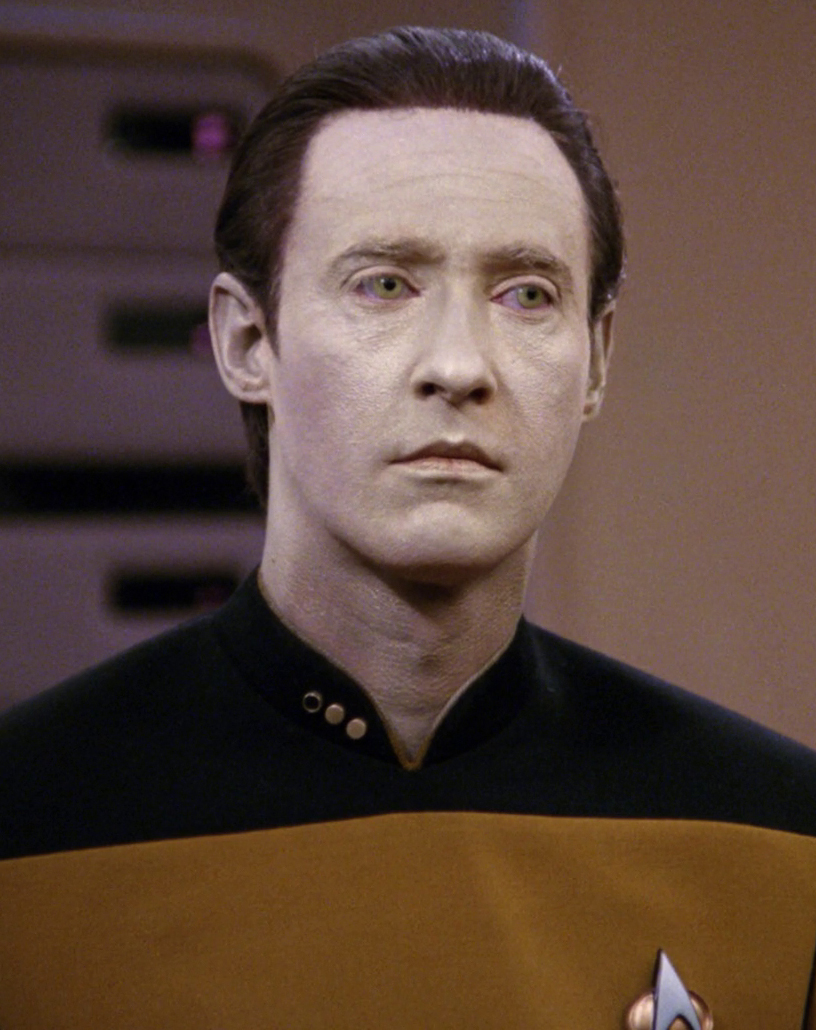
\includegraphics[width=0.4\textwidth]{images/data.jpg}
  \end{center}
\end{frame}

\begin{frame}
  \frametitle{Domains and Data}
  The two D's of software development are domains and data.
  \begin{itemize}
  \item<2-> The quantity, 5, means different things in different \emph{domains}. For a game, 4 might be the number of pixels an object should move per clock tick. For furniture website, 4 might represent the number of legs on a chair.
  \item<3-> Information in English is usually given to programmers to indicate the structure of the domain. Our job is to turn this information into \emph{data}
    representations. 
  \item<4-> After we have data representations for our domain, a program becomes a matter of data transformation.
  \item<5-> The final data produced by the program is some sort of information about our domain.
  \item<6-> If the final data is 42, this might be some height in pixels, the number of units sold, the meaning of life...etc.
  \end{itemize}
\end{frame}

\defverbatim[colored]\dataDef{
\begin{minted}{Scheme}
  ; A Temperature is a Number. 
  ; interpretation represents Celsius degrees
\end{minted}
}

\begin{frame}
  \frametitle{Data Interpretation}
  For now, we will specify the interpretation of data in comments (later we will define data types).
  \begin{itemize}
  \item<2-> We will call these data definitions. Here's an example:
  \item<3-> \dataDef
  \item<4-> This specifies that the numbers produced by our program (or function) represent Celsius degrees
  \item<5-> Such a specification rules out ``cold'' as a temperature but not -400 (which is not a real C temp)
  \item<6-> Later, we will learn to put such specifications on data, but for now our english descriptions suffice
  \end{itemize}
\end{frame}

\begin{frame}
  \frametitle{The Design Process}
  Keeping Data Interpretation in mind, let's turn to our program design process
  \begin{enumerate}
  \item<2-> Express how you wish to represent information as data. A one-line comment for specifying \emph{data interpretations} suffices.
  \item<3-> Write down a signature, a statement of purpose, and a function header.
    \begin{itemize}
    \item<4-> A \emph{signature} communicates the domain and codomain of your function. For example: \mintinline{Scheme}{; Number Number -> Number}
    \item<5-> A \emph{statement of purpose} communicates what the function produces and how it produces the answer
    \item<6-> A \emph{function header} is merely a stub definition for the function with a name, parameters, and a trivial body: \mintinline{Scheme}{(define (add x y) 0)}
    \end{itemize}    
  \end{enumerate}
\end{frame}

\defverbatim[colored]\squareExample{
\begin{minted}{Scheme}
    ; Number -> Number
    ; computes the area of a square with side len 
    ; given: 2, expect: 4
    ; given: 7, expect: 49
    (define (area-of-square len) 0)
\end{minted}
}

\defverbatim[colored]\squareTests{
\begin{minted}{Scheme}
    (sqr 2); gives: 4
    (sqr 7); gives: 49
\end{minted}
}

\begin{frame}
  \frametitle{The Design Process (cont.)}
  \begin{enumerate}
    \setcounter{enumi}{2}
  \item Create \emph{functional examples} that illustrate the expected input and output behaviors of a function. Consider a function that computes the square of a number: \squareExample
  \item<2-> \emph{Take inventory} for the program. See what is given and what needs to be computed. Basically, each function header indicates
    what is needed and then we start to skeleton the body based on the parameters:
    \begin{itemize}
    \item<3-> \mintinline{Scheme}{(define (area-of-square len) (... len ...))}
    \item<4-> The dots indicate where the function needs to be fleshed out.    
    \end{itemize}
  \end{enumerate}
\end{frame}

\begin{frame}
  \frametitle{The Design Process (cont.)}
  \begin{enumerate}
    \setcounter{enumi}{4}
  \item<2-> Now we finally \emph{code}. Based on our inventory and functional examples, we should have some idea of what to replace the ... with.
    For the program we've been discussing, our function body becomes \mintinline{Scheme}{(sqr len)}, where the second ... is removed.
  \item<3-> The final step is \emph{testing} the definition based on our functional examples.
    We'll first verify the correctness of this definition in Racket. But if we made a mistake it could be one of three kinds:
    \begin{itemize}
    \item<4-> The functional examples were wrong.
    \item<5-> The function definition was wrong and needs to be rewritten.
    \item<6-> Both the examples and the definition were wrong.
    \item<7-> In any case, we have to back and verify that steps 3 was done correctly, and if it was, then we head back to step 5. Otherwise, fix the examples and retest.
    \end{itemize}    
  \end{enumerate}
\end{frame}    


\begin{frame}
  \frametitle{Programming in Different Domains}
  There are two different kinds of domain knowledge that programmers typically deal with.
  \begin{itemize}
  \item<2-> One is knowledge from external domains. In Lafayette alone, there are programmers working on programs dealing with pharmaceutical operations, food  delivery, ambulance services, jewelry, oil field technology, insurance claims, and more. So  how do programmers figure out how to write functions
    for dealing with these different domains? One necessary skill is to learn math, which is common to many domains. The other is to learn communication skills so that you can pick up necessary skills for new domains by communicating with experts in these fields.
  \item<3-> The other domain knowledge that is used is knowledge of library functions. Knowing what things are already written for you greatly speeds up development.
    Don't reinvent the wheel.
  \end{itemize}  
\end{frame}

\begin{frame}
  \frametitle{From Functions to Programs}
  It's rare that a program consists of a single function definition unless it's trivial or poorly written. So why does the need for multiple functions arise?
  \begin{itemize}
  \item<2-> When designing an interactive program, we need separate functions for handling different events, like handling a mouse click versus a keyboard press.
  \item<3-> For batch programs, auxiliarly functions are needed when solving some subpart of the overall problem. For example, we need a function to square numbers
    when defining a batch program that computes the area of a circle when given its radius.
  \item<4-> Although not a necessity, often we encounter that the same computation is needed twice, and copying code is tedious and error-prone.
  \item<5-> For these reasons for needing functions, programmers should keep a \emph{wish list} of functions that they need to define.
  \end{itemize}
  
\end{frame}

\begin{frame}
  \frametitle{Wish Lists}
  \begin{center}
    \includegraphics[width=0.25\textwidth]{images/christmas-list.jpeg}
  \end{center}
  \begin{itemize}
  \item<2-> Here's an algorithm for writing programs with a wish list.
  \item<3-> If writing a batch program, put the main function on the list. If writing an interactive program, put the event handling functions, etc. on the wish list.
  \item<4-> Take an item off of the wish list and start designing it.
  \item<5-> When designing the function, if it seems that another function is necessary to finish the current design, then put this new function on the wish list and
    start designing it.
  \item<6-> Keep designing functions on the wish list until no more remain. After this, the program should be complete.
  \end{itemize}
\end{frame}

\begin{frame}
  \frametitle{Everyone's Favorite Activity}
  \begin{center}
    \includegraphics[width=0.4\textwidth]{images/testing.png}
  \end{center}
  \begin{itemize}
  \item<2-> Love it or hate it, testing is an essential part of software development, as we want our software to behave correctly and predictably. 
  \item<3-> Testing functions by loading the program and using the repl with manual input values is a tedious and brittle way to ensure the validity of programs.
  \item<4-> So, we want a facility to mechanize testing, which Racket (and most languages) provides.
  \item<5-> What are we waiting for? Let's get cooking (testing)!
  \end{itemize}
\end{frame}

\defverbatim[colored]\testProgram{
\begin{minted}{Scheme}
  ; Number -> Number 
  ; converts Fahrenheit temperatures to Celsius
  ; given 32, expect 0
  ; given 212, expect 100
  ; given -40, expect -40
  (define (f2c f)
    (* 5/9 (- f 32)))
\end{minted}
}

\defverbatim[colored]\tests{
\begin{minted}{Scheme}
    (check-expect (f2c -40) -40)
    (check-expect (f2c 32) 0)
    (check-expect (f2c 212) 100)
\end{minted}
}

\begin{frame}
  \frametitle{Check Your Expectations}
  Let us consider testing a Fahrenheit to Celsius conversion program:
  \testProgram
  \begin{itemize}
  \item<2-> Our tests should be created from our functional examples.
  \item<3-> Using rackets \mintinline{Scheme}{check-expect} form, we can write the appropriate tests:
    \tests
  \end{itemize}
\end{frame}

\begin{frame}
  \frametitle{Testing (cont.)}
  \begin{itemize}
  \item  The general expression \mintinline{Scheme}{(check-expect exp-to-test expected-value)} says that the expression \mintinline{Scheme}{exp-to-test}
    should evaluate to \mintinline{Scheme}{expected-value}, and otherwise the test fails.
  \item<2-> To run tests under Racket, we add the expression \mintinline{Scheme}{(test)} to our file.
  \item<3-> You can add test expressions before a function is even defined, and it will be fine.
  \item<4-> You can also test images in Dr Racket:
    \includegraphics[width=0.4\textwidth]{images/test-image.png}
  \item<5-> Write lots of tests so that you can be confident in the correctness of your programs as you develop them!
  \end{itemize}
\end{frame}

\begin{frame}
  \frametitle{How to Design Interactive Programs}
  Our previous discussion of event-driven bigbang programs was done in an ad hoc way. Now we discuss how to systematically design such programs.
  \begin{itemize}
  \item<2-> To start designing world programs, you must first create a data definition for all possible states.
  \item<3-> Then comes writing stubs for each of the event handling functions.
  \item<4-> Then the stubs for the exit and rendering functions.
  \item<5-> Putting these all together creates our wish list.
  \end{itemize}
\end{frame}

\begin{frame}
  \frametitle{An Example Wish List}
  \begin{center}
    \includegraphics[width=0.7\textwidth]{images/wish-list.png}
  \end{center}
\end{frame}

\defverbatim[colored]\constants{
\begin{minted}{Scheme}
    (define WIDTH-OF-WORLD 200) ;physical constant
    ...
    (define WHEEL
      (circle WHEEL-RADIUS "solid" "black")) ;graphical constant
\end{minted}
}

\defverbatim[colored]\worldState{
\begin{minted}{Scheme}
      ; A WorldState is a Number.
      ; interpretation the number of pixels between
      ; the left border of the scene and the car
\end{minted}
}

\begin{frame}
  \frametitle{Interactive Design By Example}
  Let's illustrate the rest of the design for an interactive program by example.
  We will have three big steps to illustrate and one small one.
  \begin{itemize}
  \item<2-> Let's animate a car moving across the screen, moving to the right 3 pixels per clock tick. 
  \end{itemize}
  \begin{enumerate}
  \item<3-> For all properties of the world that do not change, introduce constants.
    We will introduce constants for the description for the car. These are separated into two parts, graphical and physical constants:
    \constants
  \end{enumerate}
\end{frame}

\begin{frame}
  \frametitle{Interactive Design By Example (cont.)}
  \begin{enumerate}
    \setcounter{enumi}{1}
  \item<1-> Other properties do change over time and events and determine the state of the world. We must give an interpretation of what our world state means.
    \begin{itemize}
    \item<2-> So, based on our problem description what changes over time?
    \item<3-> Right, so our worldState is the position of the car:
      \worldState
    \end{itemize}
  \item<4-> After defining constants and the interpretation of our world state,
    we can start defining the relevant functions that will be on our wish list.
    \begin{itemize}
    \item<5-> Typically our wish list starts with our event handling functions, something to indicate when the program terminates, and our render function
    \item<6-> For this program, there is only 1 event that we need to handle. What is it?
    \end{itemize}
  \end{enumerate}
\end{frame}

\defverbatim[colored]\tock{
\begin{minted}{Scheme}
  ; WorldState -> WorldState
  ; adds 3 to x to move the car right 
  (define (tock x) x)
\end{minted}
}

\defverbatim[colored]\render{
\begin{minted}{Scheme}
  ; WorldState -> Image
  ; places the image of the car x pixels from 
  ; the left margin of the BACKGROUND image 
  (define (render x) BACKGROUND)
\end{minted}
}

\begin{frame}
  \frametitle{Interactive Design By Example (cont.)}
  Since the problem description doesn't specify anything about user
  input, we only have to handle clock events. Moreover, we don't have a specification that the car should stop at the right edge of the screen, so no termination function is needed. So what functions are on our wishlist that we need to apply our design process to?
  \begin{enumerate}
  \item<2-> We need a function \mintinline{Scheme}{tock} for handling clock ticks
  \item<3-> We need a function \mintinline{Scheme}{render} to draw the scene.
  \end{enumerate}
  \begin{itemize}
  \item<4-> Skeletoning out our tock function:
    \tock
  \item<5-> Our render function:
    \render
  \end{itemize}
\end{frame}

\defverbatim[colored]\mainProg{
\begin{minted}{Scheme}
; WorldState -> WorldState
; launches the program from some initial state 
(define (main ws)
   (big-bang ws
     [on-tick tock]
     [to-draw render]))
\end{minted}
}

\begin{frame}
  \frametitle{Interactive Design By Example (cont.)}
  For our final step we need to design our main function that makes
  use of our tock and render functions. The structure of main is
  straightforward from the rest of the process so far. 
  \begin{itemize}
  \item<2-> \mainProg
  \item<3-> And that's it for skeletoning out this example! First, define constants,
    second give a world state interpretation, third start defining relevant
    functions on the wishlist, and fourth define the main function as a
    big bang expression. Now we use the design process for functions to finish
    the definitions for tock and render.
  \end{itemize}
\end{frame}

\defverbatim[colored]\tockSkeleton{
\begin{minted}{Scheme}
  ;   given: 20, expect 23
  ;   given: 78, expect 81
  (define (tock ws) (... ws ...))
\end{minted}
}

\begin{frame}
  \frametitle{Interactive Design By Example (cont.)}
  Using step 4 of our design process for functions, let us give input
  and output examples for our tock function. and skeleton out the rest of the body.
  \begin{itemize}
  \item<2-> \tockSkeleton
  \item<3-> After this, we finish the body of the function as
    \mintinline{Scheme}{(define (tock ws) (+ ws 3))}
  \item<4-> Finally, we can add tests to verify the correctness of the function:
    \mintinline{Scheme}{(check-expect (tock 20) 23)} and \mintinline{Scheme}{(check-expect (tock 78) 81)}.
  \item<5-> And similarly we can use our process to finish the render function.
    For now, we move on to making an interesting modification to the program.
  \end{itemize}  
\end{frame}

\defverbatim[colored]\moveCar{
\begin{minted}[fontsize=\footnotesize]{Scheme}
  ; Number Number Number String -> Number
  ; If the mouse event is a click down,
  ; move the x-coordinate of the world state
  ; Given: 30 10 20 "button-down" Expect: 10
  ; Given: 30 10 20 "enter" Expect: 30
  ; Given: 30 10 20 "move" Expect: 30
  (define (move-car car-position x-click y-click click-kind) ...)
\end{minted}
}

\begin{frame}
  \frametitle{Real Interaction}
  Let's modify our car program so that a car can teleport to where a user clicks
  on the canvas (the x-coordinate, y won't change).
  \begin{itemize}
  \item<2-> What will we need to add to our big-bang expression to handle this
    new criteria?
  \item<3-> Right, we need to add a function for the on-click handler.
  \item<4-> But what arguments will click events pass to our function?
  \item<5-> It passes the x-coordinate, y-coordinate, and whether or not the
    mouse clicked down, was released, or was moved.
  \item<6-> So, we need something like:
    \moveCar
  \end{itemize}
\end{frame}

\defverbatim[colored]\moveCar{
\begin{minted}[fontsize=\footnotesize]{Scheme}
  (define (move-car car-position x-click y-click click-kind) 
    (cond
      [(string=? click-kind "button-down") x-click]
      [else car-position]))
\end{minted}
}

\begin{frame}
  \frametitle{Real Interaction (cont.)}
  Based on our functional examples, the body of move-car needs to be a
  conditional expression that depends on the string given:
  \begin{itemize}
  \item<2-> \moveCar
  \item<3-> Then the last thing we need to do is add:
    \mintinline{Scheme}{[on-click move-car]} to the big-bang expression.
  \item<4-> So, our modifications to this program was relatively simple. Why?
    Two reasons:
    \begin{enumerate}
    \item<5-> Our program is separated into a \emph{model} that represents
      the position of the car and the state of the world and a \emph{view}
      that renders the scene based on the model.
    \item<6-> The design recipes clearly relate a change in the problem description
      to an event that needs to be handled.
    \end{enumerate}
  \end{itemize}
\end{frame}

\end{document}
%%% Local Variables:
%%% mode: latex
%%% TeX-master: t
%%% End:
